\documentclass[tikz,border=10pt]{standalone}
% Required libraries: matrix for the H grid, fit for boxing columns, calc for math
\usetikzlibrary{matrix, fit, calc, positioning, arrows.meta}
\usepackage{amssymb, amsmath}

\begin{document}
	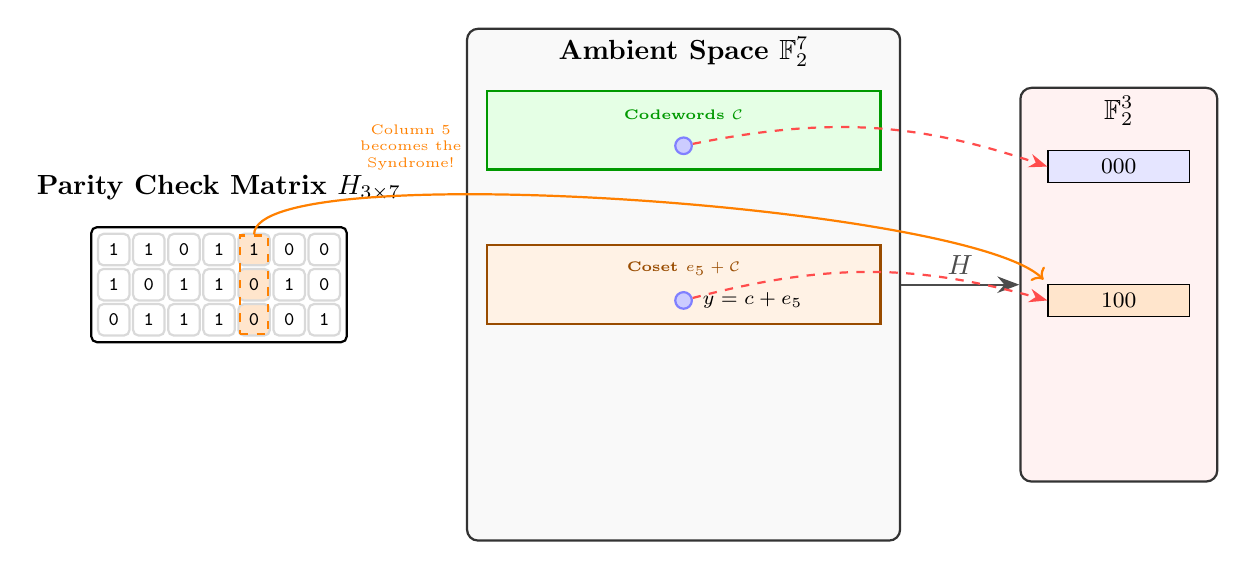
\begin{tikzpicture}[
		font=\sffamily,
		space/.style={draw=black!80, thick, rounded corners, fill=white, inner sep=10pt},
		element/.style={fill=blue!20, draw=blue!50, thick, circle, inner sep=2pt, minimum size=6pt},
		arrow/.style={-{Stealth[scale=1.2]}, thick, black!70},
		mapping/.style={-{Stealth}, dashed, thick, red!70},
		% Simplified matrix style to avoid "nodes in empty cells" errors
		bitmatrix/.style={
			matrix of nodes,
			nodes={draw=gray!30, fill=white, font=\ttfamily\scriptsize, minimum size=4mm, anchor=center},
			column sep=0.5pt, row sep=0.5pt,
			inner sep=2pt, draw=black, thick, rounded corners=2pt
		}
		]
		
		% 1. H Matrix (Manually placed to ensure no positioning errors)
		\node[font=\bfseries] (Htitle) at (0,3.2) {Parity Check Matrix $H_{3 \times 7}$};
		\matrix (H) [bitmatrix, below=0.2cm of Htitle] {
			1 & 1 & 0 & 1 & |[fill=orange!20]| 1 & 0 & 0 \\
			1 & 0 & 1 & 1 & |[fill=orange!20]| 0 & 1 & 0 \\
			0 & 1 & 1 & 1 & |[fill=orange!20]| 0 & 0 & 1 \\
		};
		
		% Use 'fit' to highlight the 5th column specifically
		\node[fit=(H-1-5)(H-3-5), inner sep=-1pt, draw=orange, thick, dashed] (col5) {};
		
		% 2. Ambient Space (F2^7)
		\node[space, right=1.5cm of H, minimum width=5.5cm, minimum height=6.5cm, fill=gray!5] (F7) {
		};
		\node[anchor=north, font=\bfseries] at (F7.north) {Ambient Space $\mathbb{F}_2^7$};
		
		% Partition slices
		\draw[draw=green!60!black, thick, fill=green!10] 
		($(F7.north) + (-2.5, -0.8)$) rectangle ($(F7.north) + (2.5, -1.8)$);
		\node[font=\tiny\bfseries, green!60!black] at ($(F7.north) + (0, -1.1)$) {Codewords $\mathcal{C}$};
		\node[element] (c) at ($(F7.north) + (0, -1.5)$) {};
		
		\draw[draw=orange!60!black, thick, fill=orange!10] 
		($(F7.center) + (-2.5, -0.5)$) rectangle ($(F7.center) + (2.5, 0.5)$);
		\node[font=\tiny\bfseries, orange!60!black] at ($(F7.center) + (0, 0.2)$) {Coset $e_5 + \mathcal{C}$};
		\node[element, label=right:{\scriptsize $y = c+e_5$}] (y) at ($(F7.center) + (0, -0.2)$) {};
		
		% 3. Syndrome Space (F2^3)
		\node[space, right=1.5cm of F7, minimum width=2.5cm, minimum height=5cm, fill=red!5] (F3) {};
		\node[anchor=north, font=\bfseries] at (F3.north) {$\mathbb{F}_2^3$};
		
		\node[draw, fill=blue!10, minimum width=1.8cm] (s0) at ($(F3.center) + (0, 1.5)$) {\footnotesize $000$};
		\node[draw, fill=orange!20, minimum width=1.8cm] (s5) at ($(F3.center) + (0, -0.2)$) {\footnotesize $100$};
		
		% Connections
		\draw[arrow] (F7.east) -- (F3.west) node[midway, above] {$H$};
		
		% Mapping arrows
		\draw[mapping] (c) to[bend left=15] (s0.west);
		\draw[mapping] (y) to[bend left=15] (s5.west);
		
		% Logic link: Col 5 is the Syndrome
		\draw[orange, thick, ->, shorten >=2pt] (col5.north) .. controls +(0,1) and +(-1,1) .. (s5.north west);
		\node[orange, font=\tiny, align=center] at ($(H.north east) + (0.8, 1)$) {Column 5\\becomes the\\Syndrome!};
		
	\end{tikzpicture}
\end{document}